\chapter{Neutrino Physics}
\label{chap:Neutrino Physics}

This chapter begins with a historical overview of neutrino flavour discoveries in \SectionRef{sec:history_of_neutrino_flavours}. Some of the key properties of neutrino physics are then discussed in \SectionRef{sec:neutrino_physics} along with the associated experiments. These include helicity, chirality, the weak interaction and neutrino oscillations. Finally, some of the experimental results that point towards the possible existence of light sterile neutrinos are described in \SectionRef{subchap:Motivation for Sterile Neutrinos} along with possible mass generation mechanisms and neutrino oscillations with the inclusion of sterile neutrino states in \SectionRef{subchap:Theory of Sterile Neutrinos}.

\section{A Brief History of Neutrino Flavours}\label{sec:history_of_neutrino_flavours}

The neutrino was first postulated in 1930 by Pauli in an attempt to explain the continuous energy spectrum observed for the electrons from beta decay experiments~\cite{Pauli_letter}. At the time it was assumed that along with the nucleus, an electron was the only other product from beta decay. That is, beta decay was thought to be a two-body decay of the form,
\begin{equation}
    {^A_Z}X \longrightarrow {^{\ \ A}_{Z+1}}Y + e^-,
\end{equation}
where \textit{X} and \textit{Y} are the elements undergoing the decay and the resultant element respectively. The continuous energy spectrum of the electron was puzzling as it was expected that the electron would always have a fixed kinetic energy and observing electrons with a range of energies appeared to violate energy conservation. Pauli theorised that in addition to the electron, a neutral particle was also emitted in beta decay and that the sum of the energy of the electron and this neutral particle would be constant \cite{Pauli_letter}.

The (electron) neutrino was not experimentally confirmed until 1956 by Cowan and Reines who used a nuclear reactor as their neutrino source \cite{cowan_and_reines_paper}. Their detector consisted of two tanks of water in which cadmium chloride had been dissolved, interlaced between three tanks of liquid scintillator. When the electron anti-neutrinos would interact with protons in one of the water tanks via inverse beta decay, a neutron and positron would be produced. The positron would then quickly annihilate with an electron producing two gamma rays. The cadmium would absorb the neutron and then emit a single gamma ray. The liquid scintillator was surrounded by \Glspl{pmt} and the signal for the experiment was two gamma rays from the electron-positron annihilation shortly followed by another gamma ray from the absorption of the neutron \cite{cowan_and_reines_paper}.

The second type of neutrino to be discovered was the muon neutrino by the Alternating Gradient Synchrotron at Brookhaven National Laboratory in 1962. The neutrinos were predominantly produced from charged pion decays which in turn were produced by firing a beam of protons at a beryllium target. The pions were directed in the direction of an iron wall during which they had the chance to decay. The iron wall was designed to absorb muons and other interacting particles. The resulting particles from neutrino interactions were then detected by an aluminium spark chamber located behind the shield. Of the selected events, the majority showed muon-like signatures (e.g. long tracks), with only a small number of events showing shower-like objects. The large disparity between the number of muon-like and electron-like events confirmed that at least two types of neutrino exist. That is the muon neutrino is distinct from the already discovered electron neutrino \cite{Muon_neutrino_discovery}. 

Following the discovery of the tau lepton in 1975 by the SLAC National Accelerator Laboratory, the tau neutrino was predicted in order to mirror the structure of the electron and muon lepton both of which have an associated neutrino \cite{tau_lepton_discovery}. The existence of the tau neutrino was eventually confirmed by the \Gls{donut} experiment in 2000. The \Gls{donut} experiment used a neutrino beam created from the decay of charmed mesons produced by protons from the  Tevatron accelerator at \gls{fermilab}. Most of the tau neutrinos were produced from the decay of the $D_s$ meson and the decay from the resulting tau lepton \cite{DONUT}.

The three confirmed flavours of neutrinos ($\nu_e, \nu_{\mu}, \nu_{\tau}$) are consistent with predictions from the \Gls{sm}. The number of expected neutrinos may be determined from the decay of the Z boson since its lifetime is dependent on the number of flavours. This was shown by the \gls{lep} experiment, which found the lifetime of the Z boson to be consistent with a three neutrino model \cite{Zboson_number_of_neutrinos}\cite{LEP}. There have, however, been results from experiments which are inconsistent with the 3 neutrino framework. Namely the excess of events observed by the \gls{lsnd} and \gls{miniboone} experiments, the deficit of events observed by the \gls{sage} and \gls{gallex} detectors (dubbed the \textit{Gallium Anomaly}) and the deficit of events observed from nuclear reactors (dubbed the \textit{Reactor Anomaly}) \cite{LSND_excess} \cite{MiniBooNE_excess} \cite{GALLEX} \cite{Gallex_reanalysis} \cite{SAGE} \cite{Reactor_anomaly}. Additional neutrino flavours may exist and not contradict the statement on the lifetime of the Z boson if they have a mass greater than half that of the Z boson and/or they do not weakly interact and hence do not contribute to the decay rate of the Z boson \cite{Zboson_number_of_neutrinos}. The hypothetical neutrinos which do not weakly interact are know as \textit{sterile} neutrinos in order to distinguish them from the \textit{active} ones that do. Sterile neutrinos will be discussed in greater detail in \SectionRef{subchap:Motivation for Sterile Neutrinos} and \SectionRef{subchap:Theory of Sterile Neutrinos}.

\section{Overview of Neutrino Physics}\label{sec:neutrino_physics}

Elementary particles are classified as either fermions or bosons depending on their spin. Fermions have odd half-integer spin whereas bosons have integer spin. Fermions are then subdivided between leptons and quarks, with one of the defining differences being that quarks experience the strong force along with the other three fundamental forces whereas the leptons only experience gravity, the weak and the electromagnetic forces. Within the \gls{sm}, bosons are subdivided into vector bosons which have a spin of one and scalar bosons which have a spin of zero \cite{Particles_and_Fundamental_Interactions:_An_Introduction_to_Particle_Physics}. The classification of elementary particles is shown in the flow chart in \FigureRef{fig:particle_classifications}.

% Flow chart made using https://www.mathcha.io
\begin{figure}[h!]
\centering

\tikzset{every picture/.style={line width=0.75pt}} %set default line width to 0.75pt        

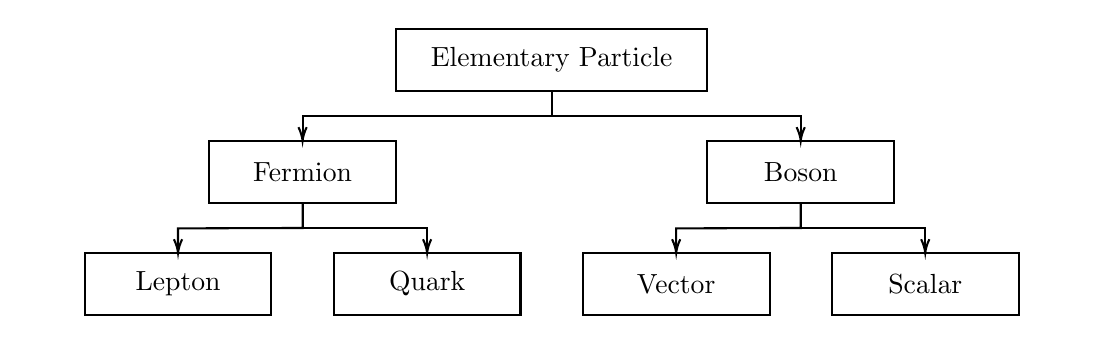
\begin{tikzpicture}[x=0.75pt,y=0.75pt,yscale=-0.6,xscale=0.6]
%uncomment if require: \path (0,306); %set diagram left start at 0, and has height of 306

%Flowchart: Process [id:dp696359542185788] 
\draw   (250,0) -- (500,0) -- (500,50) -- (250,50) -- cycle ;
%Flowchart: Process [id:dp8558192254273936] 
\draw   (100,90) -- (250,90) -- (250,140) -- (100,140) -- cycle ;
%Straight Lines [id:da09253439448016731] 
\draw    (375,50) -- (375,70) -- (175,70) -- (175,88) ;
\draw [shift={(175,90)}, rotate = 270] [color={rgb, 255:red, 0; green, 0; blue, 0 }  ][line width=0.75]    (10.93,-3.29) .. controls (6.95,-1.4) and (3.31,-0.3) .. (0,0) .. controls (3.31,0.3) and (6.95,1.4) .. (10.93,3.29)   ;
%Flowchart: Process [id:dp68005876657385] 
\draw   (500,90) -- (650,90) -- (650,140) -- (500,140) -- cycle ;
%Straight Lines [id:da33712707461320757] 
\draw    (375,50) -- (375,70) -- (575,70) -- (575,88) ;
\draw [shift={(575,90)}, rotate = 270] [color={rgb, 255:red, 0; green, 0; blue, 0 }  ][line width=0.75]    (10.93,-3.29) .. controls (6.95,-1.4) and (3.31,-0.3) .. (0,0) .. controls (3.31,0.3) and (6.95,1.4) .. (10.93,3.29)   ;
%Flowchart: Process [id:dp3110089650740445] 
\draw   (200,180) -- (350,180) -- (350,230) -- (200,230) -- cycle ;
%Flowchart: Process [id:dp3099562495446989] 
\draw   (0,180) -- (150,180) -- (150,230) -- (0,230) -- cycle ;
%Straight Lines [id:da28817746508352227] 
\draw    (175,140) -- (175,160) -- (75,160.33) -- (75,178) ;
\draw [shift={(75,180)}, rotate = 270] [color={rgb, 255:red, 0; green, 0; blue, 0 }  ][line width=0.75]    (10.93,-3.29) .. controls (6.95,-1.4) and (3.31,-0.3) .. (0,0) .. controls (3.31,0.3) and (6.95,1.4) .. (10.93,3.29)   ;
%Straight Lines [id:da0575641466520187] 
\draw    (175,140) -- (175,160) -- (275,160) -- (275,178) ;
\draw [shift={(275,180)}, rotate = 270] [color={rgb, 255:red, 0; green, 0; blue, 0 }  ][line width=0.75]    (10.93,-3.29) .. controls (6.95,-1.4) and (3.31,-0.3) .. (0,0) .. controls (3.31,0.3) and (6.95,1.4) .. (10.93,3.29)   ;
%Flowchart: Process [id:dp9199853601080596] 
\draw   (600,180) -- (750,180) -- (750,230) -- (600,230) -- cycle ;
%Flowchart: Process [id:dp3060126152626834] 
\draw   (400,180) -- (550,180) -- (550,230) -- (400,230) -- cycle ;
%Straight Lines [id:da9627421340802131] 
\draw    (575,140) -- (575,160) -- (475,160.33) -- (475,178) ;
\draw [shift={(475,180)}, rotate = 270] [color={rgb, 255:red, 0; green, 0; blue, 0 }  ][line width=0.75]    (10.93,-3.29) .. controls (6.95,-1.4) and (3.31,-0.3) .. (0,0) .. controls (3.31,0.3) and (6.95,1.4) .. (10.93,3.29)   ;
%Straight Lines [id:da7774551354270922] 
\draw    (575,140) -- (575,160) -- (675,160) -- (675,178) ;
\draw [shift={(675,180)}, rotate = 270] [color={rgb, 255:red, 0; green, 0; blue, 0 }  ][line width=0.75]    (10.93,-3.29) .. controls (6.95,-1.4) and (3.31,-0.3) .. (0,0) .. controls (3.31,0.3) and (6.95,1.4) .. (10.93,3.29)   ;

% Text Node
\draw (175,115) node   [align=left] {\begin{minipage}[lt]{102pt}\setlength\topsep{0pt}
\begin{center}
Fermion
\end{center}

\end{minipage}};
% Text Node
\draw (575,115) node   [align=left] {\begin{minipage}[lt]{102pt}\setlength\topsep{0pt}
\begin{center}
Boson
\end{center}

\end{minipage}};
% Text Node
\draw (275,205) node   [align=left] {\begin{minipage}[lt]{102pt}\setlength\topsep{0pt}
\begin{center}
Quark
\end{center}

\end{minipage}};
% Text Node
\draw (75,205) node   [align=left] {\begin{minipage}[lt]{102pt}\setlength\topsep{0pt}
\begin{center}
Lepton
\end{center}

\end{minipage}};
% Text Node
\draw (675,205) node   [align=left] {\begin{minipage}[lt]{102pt}\setlength\topsep{0pt}
\begin{center}
Scalar
\end{center}

\end{minipage}};
% Text Node
\draw (375,25) node   [align=left] {\begin{minipage}[lt]{102pt}\setlength\topsep{0pt}
\begin{center}
Elementary Particle
\end{center}

\end{minipage}};
% Text Node
\draw (475,205) node   [align=left] {\begin{minipage}[lt]{102pt}\setlength\topsep{0pt}
\begin{center}
Vector
\end{center}

\end{minipage}};
\end{tikzpicture}
\caption{Elementary particle classifications within the \gls{sm}.}
\label{fig:particle_classifications}
\end{figure}

Since neutrinos are neutral fermions, it is possible that neutrinos are their own anti-particle (a Majorana Particle). This idea was first proposed in 1937 by Majorana \cite{Majorana2020}. Within the \Gls{sm}, all fermions with the possible exception of neutrinos behave as Dirac fermions, that is, the particle and anti-particle are distinct \cite{dirac_majorana_neutrinos}. With the possibility that neutrinos are Majorana in nature, it has led to the search for neutrinoless double beta decay \cite{Double_beta_decay}. This is a variation on ordinary double beta decay in which a nucleus decays by emitting two electrons simultaneously. In ordinary double beta decay, there would also be two (anti)neutrinos in the final state, however, if neutrinos are Majorana particles, it can be thought of as one nucleon emitting a neutrino and the other absorbing it hence there are no neutrinos in the final state. Observation of such a decay would confirm the Majorana nature of neutrinos and give direct evidence for physics beyond the \Gls{sm} since the lepton number would not be conserved. Furthermore, neutrino oscillations (which is discussed in \SectionRef{subsec:Neutrino Oscillations}) are at odds with the \gls{sm} assumption that neutrinos are massless. With the requirement that neutrinos are indeed massive, the Dirac or Majorana nature of neutrinos is again discussed in \SectionRef{subsec:Neutrino Mass} within the context of mass generation mechanisms \cite{The_physics_of_neutrinos_book}.

\subsection{Helicity and Chirality}
The helicity of a particle is defined as the projection of its spin onto the linear momentum.  If the spin is aligned with the direction of motion, the particle is said to be \textit{right-handed} and has an eigenvalue equal to +1 whereas if the spin is aligned in the opposite direction a particle is said to be \textit{left-handed} and has an eigenvalue equal to -1 \cite{MartinandShaw}. It was observed by Goldhaber and others that neutrinos appear to exclusively have left-handed helicities (and right-handed helicities for anti-neutrinos). The experiment they used to determine this was as follows; consider the decay of an isomer of europium via electron capture to an excited state of samarium. The samarium nucleus then decays to its ground state by emitting a photon. 
\begin{equation}
    ^{152m}Eu + e^- \longrightarrow {^{152}Sm^*} + \nue \longrightarrow ^{152}Sm + \gamma
\end{equation}
To conserve momentum, the excited samarium nucleus must recoil in a direction opposite to the emitted neutrino. To conserve angular momentum the spin of the neutrino and the recoiling nucleus must be in opposite directions which means that they both have the same handedness. Finally, the photon emitted will have a spin in the opposite direction to the neutrino and if the photon is emitted in a direction opposite to the neutrino direction, both will have the same helicity. The photons emitted in the direction opposite to the neutrino were identified, their helicity determined and it was found that they were all left-handed \cite{Goldhaber_experiment}. 

Helicity does commute with the Hamiltonian, however, it is not Lorentz invariant (for massive particles) \cite{Introduction_to_Particle_and_Astroparticle_Physics_book}. Since massive particles travel at speeds less than \textit{c}, it is always possible to boost to a frame such that the direction of motion is reversed. Spin is not affected by this which means that it is possible for the sign of the helicity to change. In contrast to helicity, chirality is a Lorentz invariant quantity that does not commute with the Hamiltonian. The chirality operator is $\gamma^5$ and it is defined as $i\gamma^0\gamma^1\gamma^2\gamma^3$ (i.e. \textit{i} times the product of the gamma matrices). Similarly to helicity, when the chirality operator acts on the eigenfunctions $\psi_R$ and $\psi_L$ it results in an eigenvalue of +1 and -1 respectively. It is commonly expressed in term of projection operators $P_{(L, R)}$ such that,
\begin{equation}
\begin{split}
    \psi_L &= P_L\psi \isdefined \frac{1-\gamma^5}{2}\psi \\
    \psi_R &= P_R\psi \isdefined \frac{1+\gamma^5}{2}\psi,
\end{split}
\end{equation}
where $\psi$ is a spinor which can be written in terms of left and right chiral components, $\psi = \psi_L + \psi_R$.
By defining $\overline{\psi} \equiv \psi^\dag \gamma^0$ and noting that $P_{(L,R)}^\hermitianT = P_{(L,R)}$ and $P_{(L,R)}\gamma^0 = \gamma^0P_{(R,L)}$, it follows that
\begin{equation}\label{eqn:chiral identity}
    \overline{\psi_L}\psi_L = \overline{\psi_R}\psi_R = 0.
\end{equation}
It should be noted that for massless particles, helicity is Lorentz invariant and becomes identical to chirality \cite{Fundamentals_of_Neutrino_Physics_and_Astrophysics}.

\subsection{Weak Interactions and CP violation}

The weak force is mediated by the charged W$^\pm$ and neutral Z$^0$ bosons. It is dubbed \textit{weak} because if the strong or \gls{em} forces are also present the weak force is usually subdominant. The active neutrinos only interact via the weak force (and gravity) which is one of the reasons they have been historically difficult to detect. 

The weak force has two associated types of interaction: \gls{cc} interactions which are mediated by the charged W boson and \gls{nc} interactions which are mediated by the neutral Z boson. The defining difference is that for \gls{cc} interactions current flows between the interacting fermions (i.e. charge is exchanged), whereas for \gls{nc} interactions, the total flow of charge between the interacting fermions is zero. The weak component of the \gls{sm} Lagrangian is therefore comprised of two terms, one representing \gls{cc} and one representing \gls{nc}. The \gls{cc} current, $j^{CC}_{weak}$,  and \gls{nc} current, $j^{NC}_{weak}$, components of each of these terms may be expressed as, 
\begin{equation}\label{eqn:weak current}
\begin{split}
    j^{CC}_{weak} &= \frac{g}{\sqrt{2}}\overline{\psi}\gamma^{\mu}P_L\psi, \\
    j^{NC}_{weak} &= \frac{g}{2\cos{\theta_W}}\sum_{i = \nu, l}
    \overline{\psi}_i \gamma^\mu (g_V^i - g_A^i \gamma^5)\psi_i, 
\end{split}
\end{equation}
where $g$ is the weak coupling factor, $\theta_W$ is the Weinberg angle, $g_V$ is the vector coupling and $g_A$ is the axial coupling \cite{Particles_and_Fundamental_Interactions:_An_Introduction_to_Particle_Physics}\cite{Fundamentals_of_Neutrino_Physics_and_Astrophysics}\cite{PDG_2022}. The weak coupling is related to the Fermi Constant, $G_F$, and the boson masses such that,
\begin{equation}
\begin{split}
    \frac{g^2}{8m^2_W} &= \frac{G_F}{\sqrt{2}}, \\
    \frac{g^2}{8m^2_Z\cos^2{\theta_W}} &= \frac{G_F}{\sqrt{2}},
\end{split}
\end{equation}
where $m_W$ is the mass of the W boson and $m_Z$ is the mass of the Z boson \cite{Fundamentals_of_Neutrino_Physics_and_Astrophysics}.

It was shown experimentally by Wu that \gls{p} conservation is violated and later by Cronin and Fitch that \gls{cp} conservation is also violated \cite{Wu_experiment}\cite{Cronin_and_Fitch_experiment}. \gls{cp} violation is one of the Sakharov conditions required to have a matter-antimatter asymmetry in the universe, however, the amount of \gls{cp} violation seen in the quark sector is seemingly insufficient to explain the matter-dominated universe that is observed \cite{Sakharov_conditions}. There may also be \gls{cp} violation from the \gls{pmns} matrix in the lepton sector which could help explain the matter-antimatter asymmetry. However, the amount of \gls{cp} violation in the lepton sector, if any, is currently unknown \cite{leptonic_cp_violation}.  


$j^{CC}_{weak}$ has the form of a vector-axial (V--A) interaction, where the vector current is given by $\overline{\psi}\gamma^\mu\psi$ and the axial current is given by $\overline{\psi}\gamma^\mu\gamma^5\psi$. The axial component remains unchanged under a parity transformation, whereas the sign of the vector component changes. Usually, the square of the amplitude is of interest, which in short means taking the square of the weak current. This results in a squared vector and axial component plus a cross-term. Since the axial and vector components behave differently under a parity transformation, this cross term leads to parity violation \cite{Particles_and_Fundamental_Interactions:_An_Introduction_to_Particle_Physics} \cite{Fundamentals_of_Neutrino_Physics_and_Astrophysics}. $j^{NC}_{weak}$ does not have the form of a V--A interaction, but does again have both vector and axial components which lead to parity violation \cite{Particles_and_Fundamental_Interactions:_An_Introduction_to_Particle_Physics}.

\begin{comment}
Because the projection operator, $P_L$, appears in \EquationRef{eqn:weak current} it follows that weak interactions only apply to left-handed particles (and right-handed antiparticles).
\end{comment}

The \gls{sm} is constructed such that only the left components of the field couple to the W and Z bosons so it follows that only left-handed particles (and right-handed anti-particles) can weakly interact. Neutrinos only interact via the weak force which means they are therefore produced with a left-handed chirality and since they are ultra-relativistic, for all intents and purposes they also have a left-handed helicity. Additionally, a neutrino that is present in a weak interaction is always in a definite flavour state which corresponds to the associated charged lepton (therefore conserving lepton number) \cite{Quarks_and_Leptons:_An_Introductor_Course_in_Modern_Particle_Physics_book}. 

\subsection{Neutrino Oscillations}\label{subsec:Neutrino Oscillations}
Another unique property of neutrinos are their ability to oscillate. That is, the neutrino flavour may change as it propagates. This phenomenon was first proposed by Pontecorvo in 1957 \cite{Pontecorvo}. In the following years, this work was built upon by Maki, Nakagawa, Sakata and Pontecorvo himself \cite{MNS_oscillations}. 

One of the first experimental results to eventually be explained by neutrino oscillations was the Homestake experiment. This was an experiment in the 1960s that was designed to count the number of solar neutrinos. The crux of the experiment was to fill an underground tank with dry-cleaning fluid (perchloroethylene) since it contains chlorine. The solar neutrinos would be detected by inverse beta decay via
\begin{equation}
    ^{37}Cl + \nue \longrightarrow {^{37}Ar} + \electron,
\end{equation}
where the argon would be extracted and counted as it decayed. From this, the number of interacting electron neutrinos was determined, however, this number was consistently about a third of the number expected by solar predictions. This inconsistency was later dubbed the \textit{Solar Neutrino Problem} \cite{Homestake}.

The ratio of muon to electron neutrinos produced in the atmosphere from the decay of pions and muons was also studied. The predicted rate of neutrinos in the atmosphere was thought to be well understood, however a number of experiments, the most notable of which, \Gls{sk}, all observed ratios significantly below the expected value. This indicated a deficit in the observed muon neutrinos or an excess in electron neutrinos (or both). Mirroring the solar neutrino problem, these observations were dubbed the \textit{Atmospheric Neutrino Anomaly} \cite{Atmospheric_anomaly}.

In addition to measuring the ratio of atmospheric neutrinos, \Gls{sk} was also able to measure the zenith angle of the incoming neutrinos. This allowed the observed and predicted number of neutrinos to be compared as a function of the zenith angle. It was noted that the number of electron neutrinos agreed reasonably well with the expected value across all angles whereas for low-energy muon neutrinos there was a deficit of events for all angles and for high-energy muons, there was a deficit of events for zenith angles corresponding to large distances travelled (e.g. neutrinos which travelled through the earth and into the detector from below). The observed rate of high energy muons at angles corresponding to travelling directly down from the atmosphere to the detector agreed with predicted values \cite{SuperK_neutrino_oscillations}. 

The results published by \gls{sk} in 1998 allowed the atmospheric neutrino anomaly to be reconciled with neutrino oscillations and was the first time neutrino oscillations were confirmed to have been observed \cite{SuperK_neutrino_oscillations}. Shortly after, in 2001, the \Gls{sno} resolved the solar neutrino problem by again explaining the deficit in observed electron neutrinos as a result of neutrino oscillations. The \gls{sno} detector was designed with the intention of being able to measure the total neutrino flux (the sum of all three flavours) and the electron neutrino flux in isolation. The detector consisted of a tank of heavy water. Solar neutrinos have sufficient energy to interact via \gls{nc} interactions with the deuterium in the heavy water regardless of neutrino flavour,
\begin{equation}
    \nu + d \longrightarrow \nu + p + n.
\end{equation}
Neutrinos of any flavour may also interact via \gls{es},
\begin{equation}
    \nu + \electron \longrightarrow \nu + \electron.
\end{equation}
\gls{es} interactions are subdivided into \gls{cc} and \gls{nc} components, but since only \nue's are above the threshold energy for \gls{cc} interactions, there is no \gls{cc} component for \numu or \nutau. Therefore, all active neutrino flavours contribute equally to the \gls{nc} \gls{es} flux, but the flux of \nue's is enhanced due to also having a \gls{cc} component \cite{SNO_ES}. Finally, only electron neutrinos may interact via \gls{cc},
\begin{equation}
    \nue + d \longrightarrow p + p + \electron,
\end{equation}
therefore this channel only measured the flux of \nue. Confirmation that the flux of \nue was less than the flux from the \gls{nc} or \gls{es} channels coupled with the fact that the \nue flux was in agreement with previous solar neutrino experiments was sufficient to resolve the solar neutrino problem \cite{SNO_solar_neutrinos}.

Neutrino oscillations is one of the key topics in the field and this thesis. The remainder of this section will discuss the theory of neutrino oscillations. The three flavour states (\nue, \numu, \nutau) have already been established,
but it is expected that the neutrino mass states \mbox{(\nuone, \nutwo, \nuthree)} are distinct in order to explain neutrino oscillations. The flavour eigenstate of a neutrino is what is observed, however, each flavour state is a superposition of the three mass states. As a neutrino propagates, the relative phase between the mass states is continuously changing. When a neutrino then interacts, the mass states may have a relative phase that is different to that when the neutrino was created. At the point of interaction, the flavour superposition will then collapse into a single flavour and this is what is then detected. This is the mechanism which allows neutrino flavours to oscillate. 

The transformation between the flavour and mass states is expressed as
\begin{equation}\label{eqn:state transformation}
    \ket{\nu_\alpha} = \sum_k U^*_{\alpha k} \ket{\nu_k},
\end{equation}
where $\alpha$ $\in$ (e, $\mu$, $\tau$), k $\in$ (1, 2, 3) and \textit{U} is a unitary matrix. In the case of three flavour neutrino oscillations, \textit{U}, is known as the \gls{pmns} mixing matrix which is a $3 \times 3$ matrix representing the three different states \cite{Fundamentals_of_Neutrino_Physics_and_Astrophysics}. The \gls{pmns} matrix is parameterised in terms of three mixing angles ($\theta_{12}, \theta_{13}, \theta_{23}$) and a single physical \gls{cp} violating phase, \textit{$\Kronecker_{cp}$}, as
\begin{equation}
\begin{split}
U &= 
\begin{pmatrix}
U_{e1} & U_{e2} & U_{e3} \\
U_{\mu1} & U_{\mu2} & U_{\mu3}  \\
U_{\tau1} & U_{\tau2} & U_{\tau3}
\end{pmatrix} \\
&=
\begin{pmatrix}
1 & 0 & 0 \\
0 & c_{23} & s_{23}  \\
0 & -s_{23} & c_{23}
\end{pmatrix}
\begin{pmatrix}
c_{13} & 0 & s_{13}e^{-i\delta_{cp}} \\
0 & 1 & 0  \\
-s_{13}e^{i\delta_{cp}} & 0 & c_{13}
\end{pmatrix}
\begin{pmatrix}
c_{12} & s_{12} & 0 \\
-s_{12} & c_{12} & 0  \\
0 & 0 & 1
\end{pmatrix}
\end{split}
\end{equation}
where $c_{kj} = \cos{\theta_{kj}}$, $s_{kj} = \sin{\theta_{kj}}$ and the other 5 phases of the unitary matrix have been absorbed by rephasing the lepton fields.

The time-dependent Schr{\"o}dinger equation is given by
\begin{equation} \label{eqn:t.d. schrodinger}
    i \dByd{}{t}\ket{\nu_{k}(t)} = H \ket{\nu_{k}(t)},
\end{equation}
and since neutrino mass states are eigenstates of the Hamiltonian, \textit{H},  it follows that the solution to \EquationRef{eqn:t.d. schrodinger} is given by a plane wave solution 
\begin{equation}\label{eqn:plane wave soln}
    \ket{\nu_{k}(t)} = e^{-iE_{k}t} \ket{\nu_{k}}.
\end{equation}
The amplitude of a transition, $A_{\nu_\alpha \rightarrow \nu_\beta}(t)$, is defined as the projection of the final state onto the initial state, so for flavour oscillations, the amplitude is given by
\begin{equation}
    A_{\nu_\alpha \rightarrow \nu_\beta}(t) \isdefinedas \braket{\nu_\beta|\nu_\alpha(t)}.
\end{equation}
The probability of transition, $P_{\nu_\alpha \rightarrow \nu_\beta}(t)$, is then given by the absolute square of the amplitude
\begin{equation}
    P_{\nu_\alpha \rightarrow \nu_\beta}(t) = |A_{\nu_\alpha \rightarrow \nu_\beta}(t)|^2.
\end{equation}
It follows from \EquationRef{eqn:state transformation} and \EquationRef{eqn:plane wave soln} that
\begin{equation}
    \ket{\nu_\alpha(t)} = \sum_k U^*_{\alpha k} e^{-iE_kt}\ket{\nu_k}
\end{equation}
and that the transition amplitude is given by
\begin{equation}
    A_{\nu_\alpha \rightarrow \nu_\beta}(t) = \sum_k U^*_{\alpha k} U_{\beta k} e^{-iE_kt}
\end{equation}
where the fact that $\braket{\nu_j|\nu_k} = \Kronecker_{jk}$ has been used since the mass eigenstates are orthonormal. It then follows that the oscillation probability is given by
\begin{equation}
    P_{\nu_\alpha \rightarrow \nu_\beta}(t) = \sum_{k,j} U^*_{\alpha k} U_{\beta k} U_{\alpha j} U^*_{\beta j} e^{-i(E_k-E_j)t}.
\end{equation}
Under the assumption that neutrinos are relativistic, the mass state energy, $E_k$, may be expressed in terms of the neutrino energy, \textit{E},
\begin{equation}
    E_k = \sqrt{|\Vec{p}|^2 + m_k^2} \simeq E + \frac{m_k^2}{2E}.
\end{equation}
By noting that the mass splitting, $\Delta m^2_{kj}$, is defined as 
\begin{equation}
    \Delta m^2_{kj} = m_k^2 - m_j^2
\end{equation}
and that for highly relativistic particles $t \approx L$, where \textit{L} is known as the baseline (i.e. the distance the neutrino has travelled), the oscillation probability may be written as 
\begin{equation}
     P_{\nu_\alpha \rightarrow \nu_\beta}(L,E) = \sum_{k,j} U^*_{\alpha k} U_{\beta k} U_{\alpha j} U^*_{\beta j} e^{-i\frac{\Delta m^2_{kj}L}{2E}}.
\end{equation}
Finally, in a two-flavour oscillation regime, the oscillation probability may be simplified to
\begin{comment}
\begin{equation}
\begin{split}
    P_{\nu_\alpha \rightarrow \nu_\beta} &= \sin^2(2\theta)sin^2(\frac{\Delta m^2L}{4E}), \ \ \ \ \nu_\alpha \neq \nu_\beta   \\
    P_{\nu_\alpha \rightarrow \nu_\alpha} &= 1 - P_{\nu_\alpha \rightarrow \nu_\beta},
\end{split}
\end{equation}
\end{comment}
\begin{equation}
  P_{\nu_\alpha \rightarrow \nu_\beta}=\begin{cases}
    \sin^2(2\theta)\sin^2{(\frac{\Delta m^2L}{4E})}, & \nu_\alpha \neq \nu_\beta \\
    1 - \sin^2(2\theta)\sin^2{(\frac{\Delta m^2L}{4E})}, & \nu_{\alpha} = \nu_{\beta},
  \end{cases}
  \label{eqn:osc_probability}
\end{equation}
where the mixing matrix has been reduced to a rotation matrix \cite{Fundamentals_of_Neutrino_Physics_and_Astrophysics}. 

It should be noted that what neutrino experiments probe is the mass splitting and not the absolute neutrino masses. It is understood from oscillation experiments that $\Delta m_{21}^2$, known as the solar mass splitting, is equal to $7.5 \times 10^{-5}$ eV$^2$ and that $|\Delta m_{31}^2|$, known as the atmospheric mass splitting, is equal to $2.4 \times 10^{-3}$ eV$^2$. The sign of the atmospheric mass splitting is however unknown i.e. it is an open question whether $m_3$ is the heaviest or the lightest neutrino mass state. This leads to two possibilities, the so-called \textit{normal hierarchy} where the neutrino mass states increase from $m_{1 \rightarrow 2 \rightarrow 3}$ or the \textit{inverted hierarchy} where the mass states increase from $m_{3 \rightarrow 1 \rightarrow 2}$. The best fit values for oscillation parameters and the \gls{cp} violating phase from a 3-flavour neutrino framework are shown in \TableRef{table:Best fit params} for both the normal and inverted hierarchy. The numbers have been provided by the 2020 edition of the \gls{pdg} collaboration \cite{PDG_2020}. 

The nature of the neutrino hierarchy has major impacts on several areas. Within the inverted hierarchy, there is a lower bound on the Majorana mass of the electron neutrino mass. If neutrinoless double beta decay experiments can put bounds on the neutrino mass below this, the inverted hierarchy may be ruled out (under the assumption that neutrinos are Majorana in nature). Alternatively, if the inverted hierarchy is realised, neutrinoless double beta decay experiments are promising ways to determine whether neutrinos are Majorana particles or not. There are also a number of theories which predict either the normal or inverted hierarchy, so determining the hierarchy will be a strong motivator in determining the credibility of a given theory \cite{mass_hierarchy}.

\begin{figure}[h!]
    \centering
    \includegraphics[width = \largefigwidth]{figures-chap2/mass_hierarchy.jpg}
    \caption[Neutrino hierarchy.]{Diagrammatic representation of the normal hierarchy (left) and the inverted hierarchy (right). The flavour contributions to each mass state are illustrated by the different colours \cite{mass_hierarchy_image}.}
    \label{fig:my_label}
\end{figure}

\begin{table}
\begin{tabular}{l ll}
\multicolumn{1}{c}{\multirow{2}{*}{Parameter}} & \multicolumn{2}{c}{Best Fit}                                                                           \\
\multicolumn{1}{c}{} & \multicolumn{1}{c}{Normal Hierarchy} & \multicolumn{1}{c}{Inverted Hierarchy}   \\  \hline
$sin^22\theta_{12}$ & \multicolumn{1}{r}{$0.307\pm0.013$}                                        & \multicolumn{1}{r}{$0.307\pm0.013$}  \\
$sin^22\theta_{13}$ & \multicolumn{1}{r}{$(2.20\pm0.07) \times 10^{-2}$}                         & \multicolumn{1}{r}{$(2.20\pm0.07) \times 10^{-2}$} \\
$sin^22\theta_{23}$ & \multicolumn{1}{r}{$0.546\pm 0.021$}                                       & \multicolumn{1}{r}{0.539 \pm 0.022}    \\
$\Delta m^2_{21}$   & \multicolumn{1}{r}{$(7.53\pm0.18) \times 10^{-5} \text{ eV}^2$}                     & \multicolumn{1}{r}{$(7.53\pm0.18) \times 10^{-5} \text{ eV}^2$}   \\
$\Delta m^2_{32}$   & \multicolumn{1}{r}{$(2.453\pm0.033) \times 10^{-3} \text{ eV}^2$} & $(-2.536 \pm 0.034) \times 10^{-3} \text{ eV}^2$ \\
$\delta_{CP}$       & \multicolumn{1}{r}{$1.36^{+0.20}_{-0.16} \pi$ rad}                         &  \multicolumn{1}{r}{$1.36^{+0.20}_{-0.16} \pi$ rad} \\  
\end{tabular}
\caption[3-flavour neutrino best fit values.]{The best fit values for 3-flavour neutrino oscillation parameters from the 2020 \gls{pdg} \cite{PDG_2020}.}
\label{table:Best fit params}
\end{table}

\subsection{Matter Effect}
The neutrino oscillations discussed so far have assumed that the neutrinos are propagating in a vacuum. It was shown by Wolfenstein that neutrinos propagating in matter experience a potential due to coherent forward scattering with the electrons and nucleons \cite{Wolfenstein}. This potential may be thought of as an effect similar to the index of refraction in a material \cite{Fundamentals_of_Neutrino_Physics_and_Astrophysics}. Both \gls{cc} and \gls{nc} scattering may occur, however, \gls{cc} scattering may only occur for electron neutrinos whereas \gls{nc} scattering may occur for all active neutrino flavours equally. The total Hamiltonian for neutrinos propagating in matter, $H_T$, is, therefore, the vacuum Hamiltonian as seen in \EquationRef{eqn:t.d. schrodinger} plus the Hamiltonian due to the additional potential from matter effects, $H_m$. That is 
\begin{equation}
    H_T = H + H_m \text{ \hspace{1cm} with, } \begin{split}
        & H\ket{\nu_k} = E_k\ket{\nu_k} \\
        & H_m\ket{\nu_k} = V_m\ket{\nu_k},
    \end{split}
\end{equation} 
where $V_m$ is the effective potential the neutrinos are subjected to \cite{Fundamentals_of_Neutrino_Physics_and_Astrophysics}. In the three neutrino mass basis,
\begin{equation}
H_T = \frac{1}{2E} 
\begin{pmatrix}
m_1^2 & 0 & 0 \\
0 & m_2^2 & 0 \\
0 & 0 & m_3^2
\end{pmatrix}
+ U^\dag
\begin{pmatrix}
V_e & 0 & 0 \\
0 & 0 & 0 \\
0 & 0 & 0
\end{pmatrix}
U,
\end{equation}
where $V_e$ is the effective potential due to \gls{cc} scattering. It may be shown that 
\begin{equation}
    V_e = \pm \sqrt{2}G_Fn_e,
\end{equation}
where the positive value is used for neutrinos and the negative value for anti-neutrinos, $G_F$ is the Fermi constant and $n_e$ is the electron density in the medium.
The \gls{nc} component is omitted since it contributes equally to all neutrino flavours and therefore has no impact on the oscillation probability \cite{PDG_2022}. 

If only two neutrino species are considered, the mass splitting in matter, $\Delta m^2_m$, is given by 
\begin{equation}
    \Delta m_m^2 = m_{2m}^2 - m_{1m}^2 = \Delta m^2 \sqrt{(\cos{2\theta} - A/\Delta m^2)^2 + \sin^2{2\theta}},
\end{equation}
and the mixing angle in matter, $\theta_m$, is given by
\begin{equation}
    \tan{2\theta_m} = \frac{\sin{2\theta}}{\cos{2\theta} - A/\Delta m^2},
    \label{eqn:matter_mixing_angle}
\end{equation}
where $\Delta m^2$ and $\theta$ are the vacuum mass splitting and vacuum mixing angle respectively and $A \equiv 2EV_e$. The oscillation probability is the same as is shown in \EquationRef{eqn:osc_probability}, but substituting in the relevant matter mixing angle and mass splitting instead of the vacuum values. It should be noted that if $\theta = 0$, then $\theta_m = 0$, which means that oscillations in matter can only occur if oscillations in a vacuum are possible. Furthermore, if $A = \Delta m^2\cos{2\theta}$, \EquationRef{eqn:matter_mixing_angle} diverges. This critical value of \textit{A} is knowns as the \gls{msw} resonance and corresponds to $\theta_m = \pi/4$, which means that the oscillation probability is maximal. Therefore, for any non-zero vacuum oscillation probability, there exists a value of $A$ where the matter oscillation probability is a 100\% \cite{PDG_2022}. 

Another key feature of \EquationRef{eqn:matter_mixing_angle} is that the matter mixing angle depends on the sign of $\Delta m^2$. This is not the case for vacuum oscillations. Therefore, unlike vacuum oscillations, matter oscillations are one of the possible ways that the neutrino mass hierarchy may be determined \cite{mass_hierarchy_discussion}. 

\newpage
\section{Experimental Evidence for Sterile Neutrinos}\label{subchap:Motivation for Sterile Neutrinos}

\begin{comment}
\textcolor{red}{Other crap}
Cosmology: $N_{eff} = (3.046 + \Delta N_{eff})$
For any thermalised sterile neutrinos, $\Delta N_{eff} = 1, 2, 3 ...$
Measurements have $\Delta N_{eff} \sim 0$. 
So sterile neutrinos not thermalised.? Or at least suppressed
SBL steriles imply full thermalisation (why??) - so tension...
https://s3.cern.ch/inspire-prod-files-c/
c6eedeb5b3b604ca58f1a237e1b36f30
https://arxiv.org/pdf/1904.07108.pdf page 16
https://journals.aps.org/prd/pdf/10.1103/PhysRevD.104.123524
\end{comment}

There have been a number of experimental results which are not consistent with oscillations in a three-neutrino model. Most of these anomalous results can be explained by oscillations with one or more eV scale neutrinos pointing towards the existence of at least one light sterile neutrino. The experiments which have seen results seemingly in favour of eV scale sterile neutrinos will be discussed in the upcoming sections. There are however tensions between the results in favour of additional neutrino flavours and the null results from experiments such as \gls{karmen} and \gls{minos} \cite{Where_are_we_with_light_sterile_neutrinos}. The  \gls{karmen}  experiment  was  sensitive  to $\numu \rightarrow \nue$  and  $\numubar \rightarrow \nuebar$ over a baseline of 17.6 m.  No evidence of oscillations were found and a 90\% confidence level exclusion limit was placed on $\Delta m^2 > 100$ $eV^2$ with $\sin^2{2\theta} < 4\times 10^{-2}$ and $\sin^2{2\theta} < 8.5 \times 10^{-3}$ for neutrinos and anti-neutrinos respectively \cite{KARMEN}.  The \gls{minos} experiment used a predominantly muon-neutrino beam with a peak energy of 3 GeV with the near detector being at a baseline of 1.04 km.  Again, no evidence of oscillations was observed.  For a mass splitting of $\Delta m^2_{42} = 0.5$ eV$^2$, the value of $\sin^2{2\theta_{24}}$ was constrained to be less than 0.016 for a 90\% confidence level \cite{MINOS}.

\subsection{LSND}
The \gls{lsnd} experiment involved a close to 800 MeV proton beam which produced mainly $\pi^+$ and was designed to focus on the search for $\numubar \rightarrow \nuebar$ appearance where the \numubar's were a result from the decay of anti-muons which in turn were produced from the decay of at rest $\pi^+$. The detector consisted of a tank filled with 167 tons of liquid scintillator positioned 30~m from the neutrino beam source and was able to detect both Cerenkov and scintillation light. The \nuebar appearance signal was identified from the $\nuebar + p \rightarrow \positron + n$ reaction with the signature of the reaction being the energy of the \positron and the energy of a gamma as a result of neutron capture on a free proton. The \gls{lsnd} experiment observed an excess of \mbox{87.96 \pm 22.46 \pm 6.0} events from $\nuebar + p \rightarrow \positron + n$ reactions which corresponds to a 3.8$\sigma$ excess which is shown in \FigureRef{fig:LSND excess} \cite{LSND_excess}. This was the first experiment to point towards the existence of an eV-scale neutrino. 

\begin{figure}[h!]
    \centering
    \includegraphics[width = \largefigwidth]{figures-chap2/LSND_excess.png}
    \caption[LSND excess.]{The \gls{lsnd} excess as a function of the neutrino L/E value. Events require a positron in the energy range $20 < E < 60$ MeV and a likelihood ratio of > 10 that the associated gamma was correlated (i.e. $\frac{\mathcal{L}_{\gamma}(correlated)}{\mathcal{L}_{\gamma}(accidental)} > 10$) \cite{LSND_excess}.}
    \label{fig:LSND excess}
\end{figure}
\newpage

\subsection{MiniBooNE}
\gls{miniboone} collected data from the \gls{bnb} operating in both neutrino and anti-neutrino mode. The \gls{bnb} is described in detail in \SectionRef{sec:BNB}. The (anti-)neutrinos had an energy range of $200 < E_\nu < 1250$ MeV and the baseline of the experiment was 541 m. Similar to \gls{lsnd}, \gls{miniboone} was searching for  $\overset{\scriptscriptstyle(-)}{\nue}$ appearance from a predominantly $\overset{\scriptscriptstyle(-)}{\numu}$ beam. In neutrino mode, \gls{miniboone} observed an excess of 381.2\pm85.2 \gls{ccqe} events which corresponds to a 4.5$\sigma$ excess. This is shown in \FigureRef{fig:MiniBooNE excess}. Combining this with the anti-neutrino data, an excess of 460.5\pm99.0 \gls{ccqe} events (4.7$\sigma$) were observed. A two neutrino model is assumed so that a comparison with \gls{lsnd} data can be made, however, this results in the appearance and disappearance data not being compatible with one another. This may be resolved by assuming a different model to the 3+1 neutrino framework. The results are consistent with those seen by \gls{lsnd} and again point to the existence of additional neutrino flavours beyond the three predicted by the \gls{sm} \cite{MiniBooNE_excess}. 
\begin{figure}[h!]
    \centering
    \includegraphics[width = \largefigwidth]{figures-chap2/MiniBooNE_excess.png}
    \caption[MiniBooNE excess.]{The MiniBooNE excess from \nue \gls{ccqe} events. The best fit line assumed two neutrino oscillations \cite{MiniBooNE_excess}.}
    \label{fig:MiniBooNE excess}
\end{figure}
\newpage

\subsection{Gallium Anomaly}
The \textit{Gallium Anomaly} refers to the apparent deficit of electron neutrinos observed by placing radioactive sources which decay via electron capture in the solar neutrino experiments, \gls{sage} and \gls{gallex}. The \gls{gallex} experiment utilised two separate $^{51}Cr$ neutrino sources. The key measured quantity was the production of $^{71}Ge$ due to the transformation of $^{71}Ga$ via inverse beta decay. The strength of the $^{51}Cr$ neutrino sources was measured directly and via the production of $^{71}Ge$. The combined ratio of the strength of the two sources was found to be 0.93\pm0.08 \cite{GALLEX}. A later reanalysis of the results from \gls{gallex} with new technical data gave a ratio of 0.902\pm0.078 \cite{Gallex_reanalysis}. Similar to the \gls{gallex} experiment, the \gls{sage} experiment also compared the strength of a neutrino source from direct measurements and the production of $^{71}Ge$. \gls{sage} used both a $^{51}Cr$ and a $^{37}Ar$ source.  \gls{sage} observed a ratio 0.95\pm0.12 for the $^{51}Cr$ source and a ratio of $0.79^{+0.09}_{-0.10}$ for the $^{37}Ar$ source. The weighted average from the results from the two sources from \gls{sage} and the reevaluated values from the two \gls{gallex} sources is 0.88\pm0.05 \cite{SAGE}. This is consistent with a 2.3$\sigma$ significance and is consistent with \nuebar disappearance due to mixing with a sterile neutrino \cite{gallium_anomaly}.

\subsection{Reactor Anomaly}
The \textit{Reactor Anomaly} refers to the apparent deficit of anti-electron neutrinos produced from neutron-rich fission products such as $^{235}U, ^{238}U, ^{239}Pu$ and $^{241}Pu$ undergoing  $\beta$-decay. For most cases, this involves placing a detector within a 100m of a reactor and measuring the ratio of observed to predicted event rates. The average ratio is 0.943\pm0.023. It is acknowledged that the reactor fluxes may not be perfectly understood which could be the cause for such a deficit, however, it should be noted that other experiments have observed similar deficits for comparable L/E ranges \cite{Reactor_anomaly}. 

\section{Theory of Sterile Neutrinos}\label{subchap:Theory of Sterile Neutrinos}

Assuming that the mass generation of neutrinos follows similar rules to that of other Dirac mass terms, there is motivation to try and attempt to include sterile neutrinos into theoretical models since right-handed fields are required. Some of the potential options for neutrino mass generation are discussed in \SectionRef{subsec:Neutrino Mass}. The initial mass scale for sterile neutrinos is unconstrained, however, one of the more well-motivated models is the "Type 1" \textit{seesaw model} which attempts to explain the relative size of neutrino masses and points towards very heavy sterile neutrino masses ($\gg ~1$ eV). Variations of the Seesaw model have also been proposed that incorporate light sterile neutrinos \cite{White_Paper}.

\subsection{Neutrino Mass}\label{subsec:Neutrino Mass}
The \gls{sm} Lagrangian, $\mathcal{L}$, for a fermion is given by
\begin{equation}\label{eqn:SM Lagrangian}
    \mathcal{L} = \overline{\psi}(i\gamma^{\mu} \partial_{\mu} - m)\psi
\end{equation}
with the associated Euler-Lagrange equation being the Dirac equation which is given by \cite{Fundamentals_of_Neutrino_Physics_and_Astrophysics}
\begin{equation}
    (i\gamma^\mu\partial_\mu - m)\psi = 0.
\end{equation}
\subsubsection{Dirac Mass}
Within the \gls{sm} Lagrangian, the Dirac mass term is given by $m_D\overline{\psi}\psi$ where $\psi$ is the Dirac spinor. By dividing this into left and right components it follows that
\begin{equation}\label{eqn:Dirac mass term}
\begin{split}
    m_D\overline{\psi}\psi &= m_D(\overline{\psi_L + \psi_R})(\psi_L + \psi_R) \\
    &= m_D(\overline{\psi_L}\psi_R + \overline{\psi_R}\psi_L),
\end{split}
\end{equation} 
where the second step follows from \EquationRef{eqn:chiral identity}. Naturally, to have a non-zero Dirac mass term, particles require a left and right-handed chiral state. This is the mass generation method that all particles in the \gls{sm} follow and hence why neutrinos are massless in the \gls{sm}. To give the neutrino mass in this way, a field associated with a right-handed neutrino could be introduced. This would usually correspond to the left-handed neutrinos being the \textit{active} ones, whilst the right-handed neutrinos would be considered \textit{sterile}.
\begin{comment}
Since left handed particles form a doublet under \SUgroup2 they have non-zero weak isospin and because right handed particles are a singlet under \SUgroup2, their weak isospin is equal to zero. Therefore, in order to get a term where the isospin sums to zero, which is a requirement for the Lagrangian to be gauge invariant, an additional field is needed that is also a doublet under \SUgroup2. This field is a result of the neutral Higgs boson, $\phi^0$, and the Dirac mass is given by
\end{comment}
In order for the mass terms to actually acquire mass, the \gls{sm} requires two scalar fields to be introduced. These fields are provided by the Higgs mechanism and allow for spontaneous symmetry breaking \cite{peskin_and_schroeder}. The Dirac mass is given by, 
\begin{equation}
    {m_D}_i = \frac{y_iv}{\sqrt{2}},
\end{equation}
where \textit{y} is the Yukawa coupling and \textit{v} gives the vacuum expectation value from the Higgs field ($v \simeq$ 246 GeV). A concern with generating neutrino masses in this way is the required size of the Yukawa coupling. To generate a mass of say 0.1 eV, the Yukawa coupling would need to be very small ($\sim$6 orders of magnitude less than that of the electron). This small number is sometimes considered unnatural and provides motivation to search for alternative mass mechanisms to explain the neutrino masses \cite{Fundamentals_of_Neutrino_Physics_and_Astrophysics}.

\subsubsection{Majorana Mass}
To generate mass without the requirement of a right-handed field, it is required that the neutrino be a Majorana particle. It may be shown that 
\begin{equation}
    P_R C\overline{\psi_L}^T = C\overline{\psi_L}^T,
\end{equation}
which means that $C\overline{\psi_L}^T$ is a right handed object, where the superscript \textit{T} indicates the transpose and $C = i \gamma^2 \gamma^0$ which is the charge conjugation operator. By defining $\psi_L^C = C\overline{\psi_L}^T$, the Majorana field mass term in the Lagrangian can be written as
\begin{equation}\label{eqn:Majorana mass term}
    \frac{m_L}{2}(\overline{\psi_L^C}\psi_L + \overline{\psi_L^{\phantom{C}}}\psi_L^C), 
\end{equation}
where the factor of 1/2 arises due to double counting. As is the case for the Dirac mass, the \gls{sm} requires the introduction of additional fields to allow for spontaneous symmetry breaking \cite{Fundamentals_of_Neutrino_Physics_and_Astrophysics}. 

\subsubsection{Seesaw mechanism}\label{sec:seesaw_mechanism}
If both Dirac and Majorana mass terms are present, the mass component of the Lagrangian, $\mathcal{L}_{mass}$, may be written as a matrix equation. For one active and one sterile neutrino, this has the form
\begin{comment}
In the general case, there are four neutrino fields, a left and right handed one plus a charge conjugate version of each. This allows us to create a left and right Majorana mass term akin to \EquationRef{eqn:Majorana mass term} and a regular and charge conjugated Dirac mass akin to \EquationRef{eqn:Dirac mass term} (the Dirac mass, $m_D$ is the same in both cases). The mass component of the Lagrangian, $L_{mass}$, may be written as a matrix equation, \end{comment}

\begin{equation}
    \mathcal{L}_{mass} = \frac{1}{2} 
    \begin{pmatrix}
    \overline{\psi_L^C} & \overline{\psi_R^{\phantom{C}}}
    \end{pmatrix}
    \begin{pmatrix}
    m_L & m_D \\
    m_D & m_R
    \end{pmatrix}
    \twomatrix {\psi_L} {\psi_R^C} + h.c.
\end{equation}
where the central $4 \times 4$ matrix is known as the mass matrix, $\mathcal{M}$ \cite{White_Paper}. By diagonalising $\mathcal{M}$ into mass eigenstates, $m_1, m_2$, and assuming $m_L = 0$ (since it is not allowed in the \gls{sm}) and that $m_R \gg m_D$, the mass eigenvalues may be expressed as
\begin{equation}
\begin{split}
    m_1 \simeq \frac{m_D^2}{m_R} \\
    m_2 \simeq m_R.
\end{split}
\end{equation}
Since $m_R \gg m_D$, $m_2$ is also large and $m_1$ is small since the value of $m_D^2$ is suppressed by the large value of $m_R$ in the denominator. Furthermore, the larger the value of $m_2$, the smaller the value of $m_1$. This linked relationship gives rise to the so-called Type I \footnote{A number of other seesaw mechanisms exist which typically involve the exchange of a particle such as a heavy Majorana neutrino as is the case in the Type I mechanism \cite{White_Paper}.} \textit{seesaw mechanism}. $m_1$ would give the mass scale of the active neutrinos whereas $m_2$ would be a heavy sterile neutrino. This mechanism requires neutrinos to be Majorana particles, but can be extended to include three active neutrinos and an arbitrary number of sterile neutrinos and does provide an explanation of the relative smallness of the neutrino masses compared with other \gls{sm} particles \cite{Fundamentals_of_Neutrino_Physics_and_Astrophysics}. 


\subsection{Sterile Neutrino Oscillations}\label{sec:sterile_neutrino_oscillations}
An overview of the physics describing neutrino oscillations within the active sector was presented in \SectionRef{subsec:Neutrino Oscillations}. This approach may be extended to include an arbitrary number of additional neutrino states by expanding the \gls{pmns} matrix to include the desired number of sterile neutrinos

\begin{equation}
U_{sterile} = 
\begin{pmatrix}
U_{e1} & U_{e2} & U_{e3} & U_{e4} & \dots\\
U_{\mu1} & U_{\mu2} & U_{\mu3} & U_{\mu4} & \dots \\
U_{\tau1} & U_{\tau2} & U_{\tau3} & U_{\tau4} & \dots \\
U_{s1} & U_{s2} & U_{s3} & U_{s4} & \dots \\
\vdots & \vdots & \vdots & \vdots & \ddots \\
\end{pmatrix}.
\end{equation}
For simplicity, often only the case with one sterile neutrino is considered. This is known as the $(3 + 1)$ neutrino framework which takes into account the three usual active neutrinos with the addition of one sterile neutrino. Within a $(3 + 1)$ framework and assuming that $\Delta m^2_{41} \gg |\Delta m^2_{31}|, \Delta m^2_{21}$, short baseline oscillation are well represented by the two flavour oscillation probability,

\begin{equation}
    P_{\nu_\alpha \rightarrow \nu_\beta} = \Kronecker_{\alpha \beta} -4|U_{\alpha \beta}|^2 (\Kronecker_{\alpha \beta} -|U_{\alpha \beta}|^2)\sin^2{\left(\frac{\Delta m^2_{41}L}{4E} \right)},
\label{eqn:sterile_osc_prob}
\end{equation}
where $\delta_{\alpha\beta}$ is the Kronecker delta between states $\alpha$ and $\beta$, $U_{\alpha \beta}$ are the relevant entries from the \gls{pmns} matrix and $\Delta m^2_{41}$ is the mass splitting involving the sterile neutrino state \cite{SBN_paper}. 

When performing a search for sterile neutrinos, typically there are three channels, one or more of which may be probed (plus their corresponding anti-neutrino variants). For each of these channels, the relevant \gls{pmns} matrix elements are parameterised in terms of mixing angles such that,
\begin{equation}
\centering
    &\text{\numu disappearance } (\numu \rightarrow \numu) &: \sin^2{2\thetamumu} &\isdefinedas 4|U_{\mu 4}|^2(1 - |U_{\mu 4}|^2) \label{eqn:sinsq2thmumu}\\
    &\text{\nue appearance } (\numu \rightarrow \nue) &: \sin^2{2\thetamue} &\isdefinedas 4|U_{\mu 4}|^2|U_{e4}|^2 \label{eqn:sinsq2thmue} \\
    &\text{\nue disappearance } (\nue \rightarrow \nue) &: \sin^2{2\thetaee} &\isdefinedas 4|U_{e 4}|^2(1 - |U_{e4}|^2).
    \label{eqn:sinsq2thee}
\end{equation}
It should be noted that \nue appearance depends on $U_{\mu 4}$ and $U_{e4}$, which \numu and \nue disappearance depend on respectively. The observation of \nue appearance would therefore automatically imply that \numu and \nue disappearance is also present. Additionally, this allows these parameters to be over-constrained \cite{SBN_paper}. The current global best fit values for the three mixing angles and the mass splitting term, $\Delta m^2_{41}$ are outlined in \TableRef{table:sterile_best_fit_params}.

\begin{table}[h!]
\begin{tabular}{c cc}
Oscillation Parameter        & \begin{tabular}[c]{@{}c@{}} Best Fit Value\end{tabular} \\ \hline

$\sin^2{2\theta_{\mu\mu}}$ & 0.07157      \\
$\sin^2{2\theta_{\mu e}}$ & 0.0009809      \\
$\sin^2{2\theta_{ee}}$ & 0.05310      \\
$\Delta m^2_{41}$ & 1.32 eV$^2$     \\

\end{tabular}
\caption[Best fit value for sterile oscillation parameters.]{The global best fit values for the $(3 + 1)$ sterile neutrino oscillation parameters \cite{Where_are_we_with_light_sterile_neutrinos}.}
\end{table}\label{table:sterile_best_fit_params}




%\begin{fmffile}{diagram}
%\begin{fmfgraph*}(200,150)
%    \fmfleft{i1,i2}
%    \fmfright{o1,o2}
%    \fmf{fermion, label=p/n}{i1,v1}
%    \fmf{fermion, label=n/p}{v1,o1}
%    \fmf{fermion, label=$\nu$}{i2,v2}
%    \fmf{fermion, label.side=left, label=l}{v2,o2}
%    \fmf{photon, label=$W$}{v1,v2}
%    %\fmflabel{$v_1$}{v1}
%    %\fmflabel{$v_2$}{v2}
%\end{fmfgraph*}
%\end{fmffile}



